
% \titlegraphic{\hfill\includegraphics[height=1.5cm]{logo.pdf}}

\documentclass[xcolor=pdftex,dvipsnames,table,numbers,hyperref={pdfpagelabels=false},compress]{beamer}
%\usepackage{requiredPackage}
\usepackage{amsmath}
\usepackage{graphicx}
\usepackage{amsfonts}
\usepackage{amssymb}

\usepackage{tabularx}
\usepackage{epstopdf}
\usepackage{overpic}
\usepackage{url}
\usepackage{calrsfs}
\usepackage{mathrsfs}
\usepackage{epsfig}
\usepackage{cancel}
\usepackage{changepage}

\usepackage{tikz}
\usepackage[customcolors]{hf-tikz} 

\usepackage{lmodern}
%\usepackage{mystyle}
\usepackage{subfig}
\usepackage{pifont}
\usepackage{tabu}
\usepackage{xcolor}
\usepackage{algorithm}
\usepackage{algpseudocode}
%\usepackage{enumitem}
\usepackage{remreset}
\usepackage{etoolbox}
\usepackage{comment} % end and begin comment
%\usepackage{dtklogos} 
\usepackage{listings}
\lstset{breaklines=true} 

\newcommand{\gline}{\textcolor{gray}{\hline}}
\newcommand{\cmark}{\ding{51}}%
\newcommand{\xmark}{\ding{55}}%
\newcommand{\gcheck}{\textcolor{blue}{\Large \cmark}}
\newcommand{\rcross}{\textcolor{red}{\Large \xmark}}
\newcommand{\tkt}{\tilde{K}_\theta}
\newcommand{\kt}{K_\theta}
\newcommand{\ind}{\overset{ind}{\sim}}
\newcommand{\plim}{\overset{p}{\rightarrow}}
\newcommand{\cx}{\frac {X'X}n}
\newcommand{\cz}{\frac {Z'Z}n}
\newcommand{\ccz}{\frac {Z'Z}n - \Sigma_A}
\newcommand{\czy}{\frac {Z'y}n}
\newcommand{\cyz}{\frac {y'Z}n}
\newcommand{\cxy}{\frac {X'y}n}
\newcommand{\cyx}{\frac {y'X}n}
\newcommand{\myitem}{\vskip3mm \item}

\newcommand{\calS}{{\cal S}}
\newcommand{\calA}{{\cal A}}
\newcommand{\calK}{{\cal K}}
\newcommand{\calX}{{\cal X}}
\newcommand{\calD}{{\cal D}}
\newcommand{\calG}{{\cal G}}
\newcommand{\calT}{{\cal T}}
\newcommand{\calU}{{\cal U}}
\newcommand{\calR}{{\cal R}}
\newcommand{\tp}{\tilde{p}}
\newcommand{\tildebC}{\tilde{\bC}}
\newcommand{\calL}{{\cal L}}

\newcommand{\blam}{ \mbox{\boldmath $ \lambda $} }
\newcommand{\bet}{ \mbox{\boldmath $ \eta $} }
\newcommand{\bome}{ \mbox{\boldmath $ \omega $} }
\newcommand{\bbet}{ \mbox{\boldmath $ \beta $} }
\newcommand{\bbeta}{ \mbox{\boldmath $ \beta $} }
\newcommand{\balph}{ \mbox{\boldmath $ \alpha $} }
\newcommand{\balpha}{ \mbox{\boldmath $ \alpha $} }
\newcommand{\bphi}{ \mbox{\boldmath $\phi$}}
\newcommand{\bzeta}{ \mbox{\boldmath $\zeta$}}
\newcommand{\bkap}{ \mbox{\boldmath $\kappa$}}
\newcommand{\bkappa}{ \mbox{\boldmath $\kappa$}}
\newcommand{\beps}{ \mbox{\boldmath $\epsilon$}}
\newcommand{\bepsilon}{ \mbox{\boldmath $\epsilon$}}
\newcommand{\bthet}{ \mbox{\boldmath $ \theta $} }
\newcommand{\btheta}{ \mbox{\boldmath $ \theta $} }
\newcommand{\blambda}{ \mbox{\boldmath $ \lambda $} }
\newcommand{\bnu}{ \mbox{\boldmath $\nu$} }
\newcommand{\bmu}{ \mbox{\boldmath $\mu$} }
\newcommand{\bGam}{ \mbox{\boldmath $\Gamma$} }
\newcommand{\bSig}{ \mbox{\boldmath $\Sigma$} }
\newcommand{\bSigma}{ \mbox{\boldmath $\Sigma$} }
\newcommand{\bPhi}{ \mbox{\boldmath $\Phi$} }
\newcommand{\bThet}{ \mbox{\boldmath $\Theta$} }
\newcommand{\bTheta}{ \mbox{\boldmath $\Theta$} }
\newcommand{\bDel}{ \mbox{\boldmath $\Delta$} }
\newcommand{\bDelta}{ \mbox{\boldmath $\Delta$} }
\newcommand{\bnabla}{ \mbox{\boldmath $\nabla$} }
\newcommand{\bLam}{ \mbox{\boldmath $\Lambda$} }
\newcommand{\bLambda}{ \mbox{\boldmath $\Lambda$} }
\newcommand{\bgam}{ \mbox{\boldmath $\gamma$} }
\newcommand{\bgamma}{ \mbox{\boldmath $\gamma$} }
\newcommand{\brho}{ \mbox{\boldmath $\rho$} }
\newcommand{\bdel}{ \mbox{\boldmath $\delta$} }
\newcommand{\bdelta}{ \mbox{\boldmath $\delta$} }
\newcommand{\sis}{\sigma^2}
\newcommand{\bOmega}{\mbox{\boldmath $\Omega$} }
\newcommand{\bPsi}{ {\boldsymbol \Psi} }
\newcommand{\btkt}{\boldsymbol{\tilde{K}}_\theta}
\newcommand{\pg}{P{\'o}lya-Gamma }

\newcommand{\bzero}{\textbf{0}}
\newcommand{\bones}{\textbf{1}}
\newcommand{\ba}{\textbf{a}}
\newcommand{\bb}{\textbf{b}}
\newcommand{\bB}{\textbf{B}}
%\newcommand{\bA}{\textbf{A}}
\newcommand{\bc}{\textbf{c}}
\newcommand{\bC}{\textbf{C}}
\newcommand{\bA}{\textbf{A}}
\newcommand{\bd}{\textbf{d}}
\newcommand{\bD}{\textbf{D}}
\newcommand{\be}{\textbf{e}}
\newcommand{\bE}{\textbf{E}}
\newcommand{\bk}{\textbf{k}}
\newcommand{\bK}{\textbf{K}}
\newcommand{\bh}{\textbf{h}}
\newcommand{\bs}{\textbf{s}}
\newcommand{\bS}{\textbf{S}}
\newcommand{\bH}{\textbf{H}}
\newcommand{\bI}{\textbf{I}}
\newcommand{\bt}{\textbf{t}}
\newcommand{\bu}{\textbf{u}}
\newcommand{\bv}{\textbf{v}}
\newcommand{\bw}{\textbf{w}}
\newcommand{\bW}{\textbf{W}}
\newcommand{\bx}{\textbf{x}}
\newcommand{\bX}{\textbf{X}}
\newcommand{\by}{\textbf{y}}
\newcommand{\bY}{\textbf{Y}}
\newcommand{\bz}{\textbf{z}}
\newcommand{\bZ}{\textbf{Z}}
\newcommand{\bL}{\textbf{L}}
\newcommand{\br}{\textbf{r}}
\newcommand{\bR}{\textbf{R}}
\newcommand{\bm}{\textbf{m}}
\newcommand{\bM}{\textbf{M}}
\newcommand{\given}{\,|\,}
\newcommand{\T}{\top}
\newcommand{\bV}{\textbf{V}}
\newcommand{\bJ}{\textbf{J}}
\newcommand{\blue}[1]{{\color{RoyalBlue!90} #1}}
\newcommand{\red}[1]{{\color{Red} #1}}
\newcommand{\green}[1]{{\color{Green} #1}}
\newcommand{\orange}[1]{{\color{Orange} #1}}
\newcommand{\titl}[1]{{\begin{large}\begin{center}#1\end{center}\end{large}}}

\newcommand{\tildea}{\tilde{a}}
\newcommand{\tildeba}{\tilde{\ba}}
\newcommand{\tildebv}{\tilde{\bv}}
\newcommand{\tildev}{\tilde{v}}
\newcommand{\tildeA}{\tilde{A}}
\newcommand{\tildeC}{\tilde{C}}
\newcommand{\tildeK}{\tilde{K}}
\newcommand{\tildew}{\tilde{w}}
\newcommand{\tildeu}{\tilde{u}}
\newcommand{\tildebw}{\tilde{\bw}}
\newcommand{\tildeeps}{\tilde{\epsilon}}
\newcommand{\tildebeps}{\tilde{\bepsilon}}
\newcommand{\eps}{\epsilon}
\newcommand{\sigs}{\sigma^2}
\newcommand{\taus}{\tau^2}
\newcommand{\iid}{\stackrel{\mathrm{iid}}{\sim}}

%\newcommand{\calS}{{\cal S}}
\newcommand{\calC}{{\cal C}}

%\documentclass[10pt]{beamer}

\usetheme{metropolis}
\usepackage{appendixnumberbeamer}

\usepackage{booktabs}
\usepackage[scale=2]{ccicons}

\usepackage{pgfplots}
\usepgfplotslibrary{dateplot}

\usepackage{xspace}
\newcommand{\themename}{\textbf{\textsc{metropolis}}\xspace}

\makeatletter
\@addtoreset{subfigure}{framenumber}% subfigure counter resets every frame
\makeatother

\makeatletter
\@addtoreset{figure}{framenumber}% subfigure counter resets every frame
\makeatother

\setbeamertemplate{caption}{\raggedright\insertcaption\par}
\captionsetup[subfigure]{labelformat=empty}


\title[]{Application of Spatially-Varying Coefficient Models}
\author{Jeffrey Doser$^1$ \& Andrew Finley$^2$}
	
\institute{
\begin{tiny}$^1$Department of Integrative Biology, Michigan State University.\\
$^2$Department of Forestry, Michigan State University.\end{tiny}
}

\date{May 15, 2023}


\begin{document}

\maketitle

\begin{frame}{Spatially-Varying Coefficient Models}
     \begin{itemize}
          \item Extension of spatial regression approaches that allow regression coefficients to vary across space, and not just the intercept
	  \item SVC models are random slopes models, with spatial structure given to the random slopes
     \end{itemize}
\end{frame}


\begin{frame}{SVC GLMMs}
    \begin{align*}
	    y(\bs_i) &\sim f(\mu(\bs_i), \tau) \\
	    \mu(\bs_i) &= g^{-1}(\eta(\bs_i)) = \bx(\bs_i)^\top \tilde{\bbeta}(\bs_i) \\
	    \tilde{\beta}_r(\bs_i) &= \beta_r + \text{w}_r(\bs_i) \text{ for each } r = 1, \dots, p
    \end{align*}
    \begin{itemize}
        \item We can model $\textbf{w}(\bm{s}_i)$ using a GP, predictive process, or \red{NNGP}
        \item We can envision modeling $\textbf{w}(\bm{s}_i)$ in two ways: 
        \begin{enumerate}
		\item Multivariate NNGP (see previous forest biomass example) 
		\item \red{Independent NNGPs}
        \end{enumerate}
	\item Here we focus on the latter
        \item Pros and cons to both approaches, similar to correlations between random slopes and intercepts in mixed models
    \end{itemize}
\end{frame}

\begin{frame}{Potential benefits of SVC models}
    \begin{itemize}
         \item Improved predictive performance
         \item Tremendous flexibility to accommodate spatial variability in effects
         \item Hypothesis testing and generation
         \item Accommodate highly non-linear relationships
	 \item Model spatial variability in trends over time
    \end{itemize}

\end{frame}

\begin{frame}{Improved predictive performance}
\begin{figure}[]
\begin{center}
\vskip -5mm
\subfloat[Observed biomass]{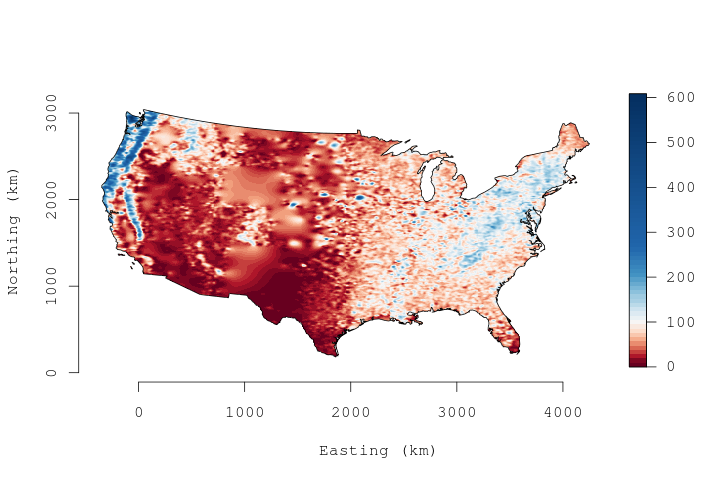
\includegraphics[width=5cm]{../figures/obs-biomass.png}\label{bio-obs}}
\subfloat[Fitted biomass]{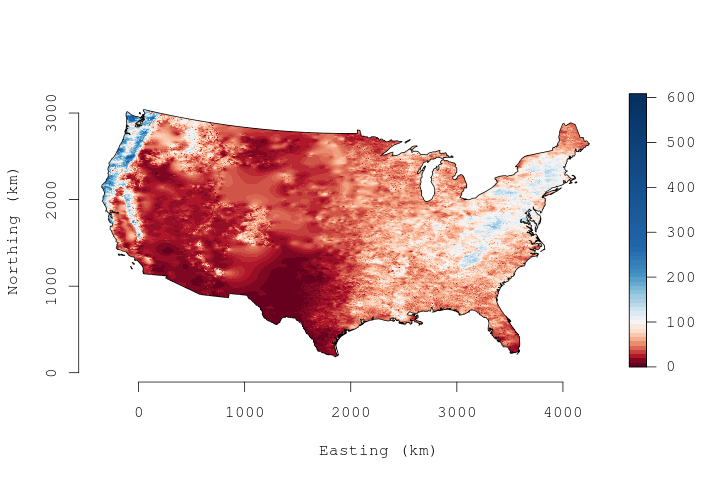
\includegraphics[width=5cm]{../figures/fitted-biomass.png}\label{bio-fitted}}\\  \vskip-2.5mm
\subfloat[$\beta_0(s)$]{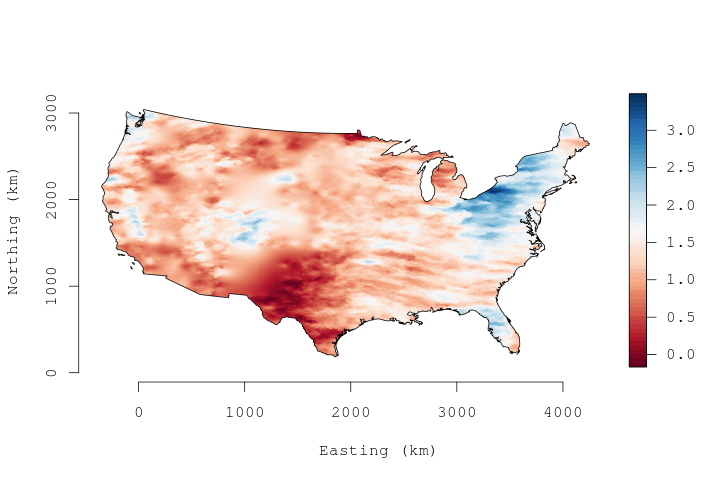
\includegraphics[width=5cm]{../figures/svc-beta0.png}\label{bio-coefs-b0}}
\subfloat[$\beta_{NDVI}(s)$]{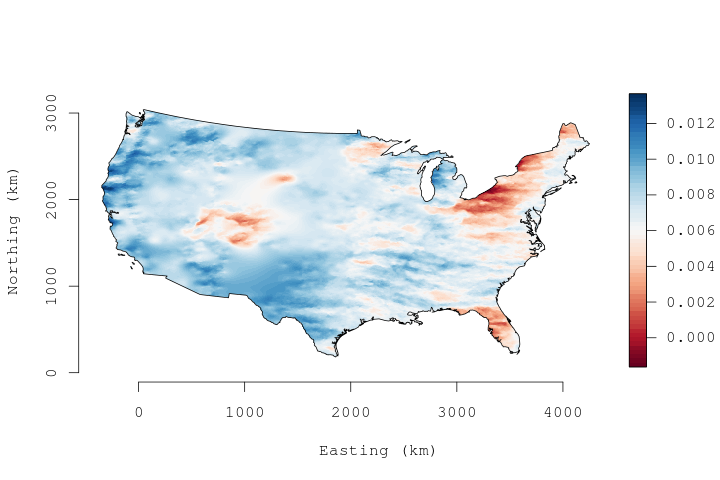
\includegraphics[width=5cm]{../figures/svc-beta1.png}\label{bio-coefs-b1}}\\
\end{center}
\label{fig:bio-coefs}
\end{figure}


\end{frame}
	
\begin{frame}{More flexibility to accommodate spatial variability in effects}

Gray Catbird occurrence trend across the eastern US from 2000-2019

\begin{center}
   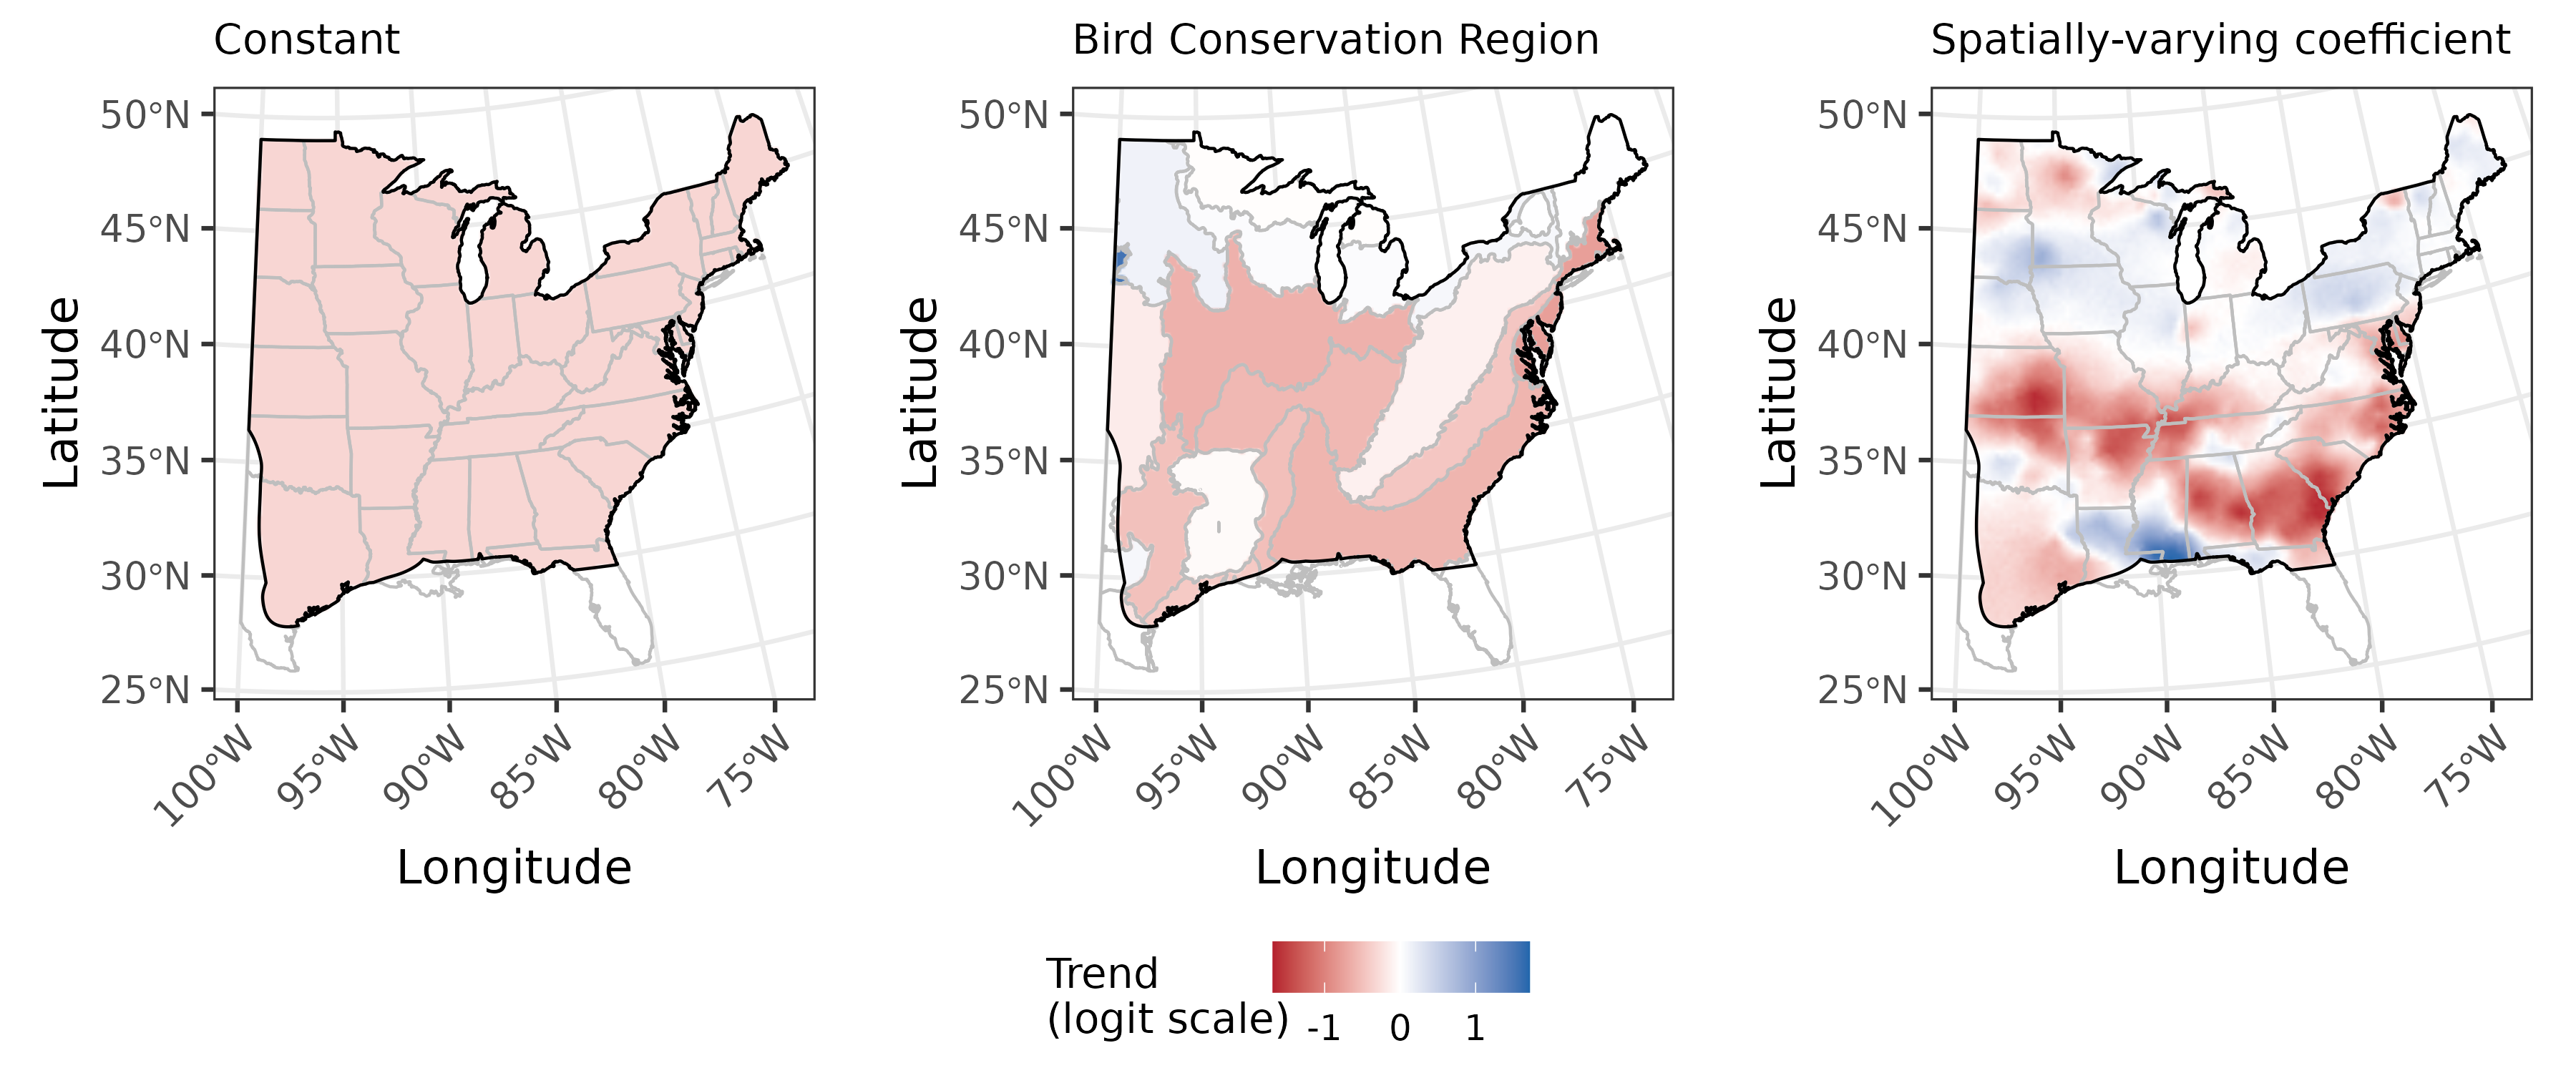
\includegraphics[width=11cm]{../figures/DKFSWZ22-GRCA-plot.png}
\end{center}
\end{frame}

\begin{frame}{Some cautionary notes: (1) Standardization of covariates}
     \begin{itemize}
          \item Common recommendation to center and scale covariates is likely not appropriate. Why? \pause
	  \item Consider a single SVC $\text{w}(\bs_i)$: \pause
               \begin{itemize}
		       \item $\text{var}(\text{w}(\bs_i)) = \text{x}^2(\bs_i)\sigma^2 + \tau^2$ \pause
		       \item $\text{cov}(\text{w}(\bs_i), \text{w}(\bs_j)) = \sigma^2\text{x}(\bs_i)\text{x}(\bs_j)\rho(\mid\bs_i - \bs_j\mid; \phi)$ \pause
		       \item If x takes both positive and negative values, variance will be high at large and small x values and small around zero. \pause
		       \item Further, negative covariances can arise, which may drive $\sigma^2$ to be very close to zero. \pause
               \end{itemize}
       \item Recommendation following Gelfand et al. (2003) \textit{JASA}: only use positive covariate values. Can lead to identifiability problems.
       \item For modeling spatially-varying trends, standardiziation is recommended. 
     \end{itemize}
\end{frame}

\begin{frame}{Some cautionary notes: (2) Inference}
	\begin{itemize}
             \item Estimating multiple GPs simultaneously is difficult.
	     \item Use caution when making inference from SVC models, particularly with observational data. \pause
	     \item The model only identifies the product of $\tilde{\beta}(\bs_i)$ and $\text{x}(\bs_i)$. Prediction at $\bs_i$ with a new covariate value (e.g., $\text{x}^\ast(\bm{s}_i)$) may not be appropriate. \pause
	     \item Recommend plotting spatial maps of SVC effects together with a plot of the covariate vs. the predicted mean for all observed locations
	     \item Interpretation can be difficult when both the effect and the covariate vary over space. More straightforward with something like a trend.
	\end{itemize}
\end{frame}

\begin{frame}{Example: Effect of max temperature on Bobolink occurrence}

\begin{center}
   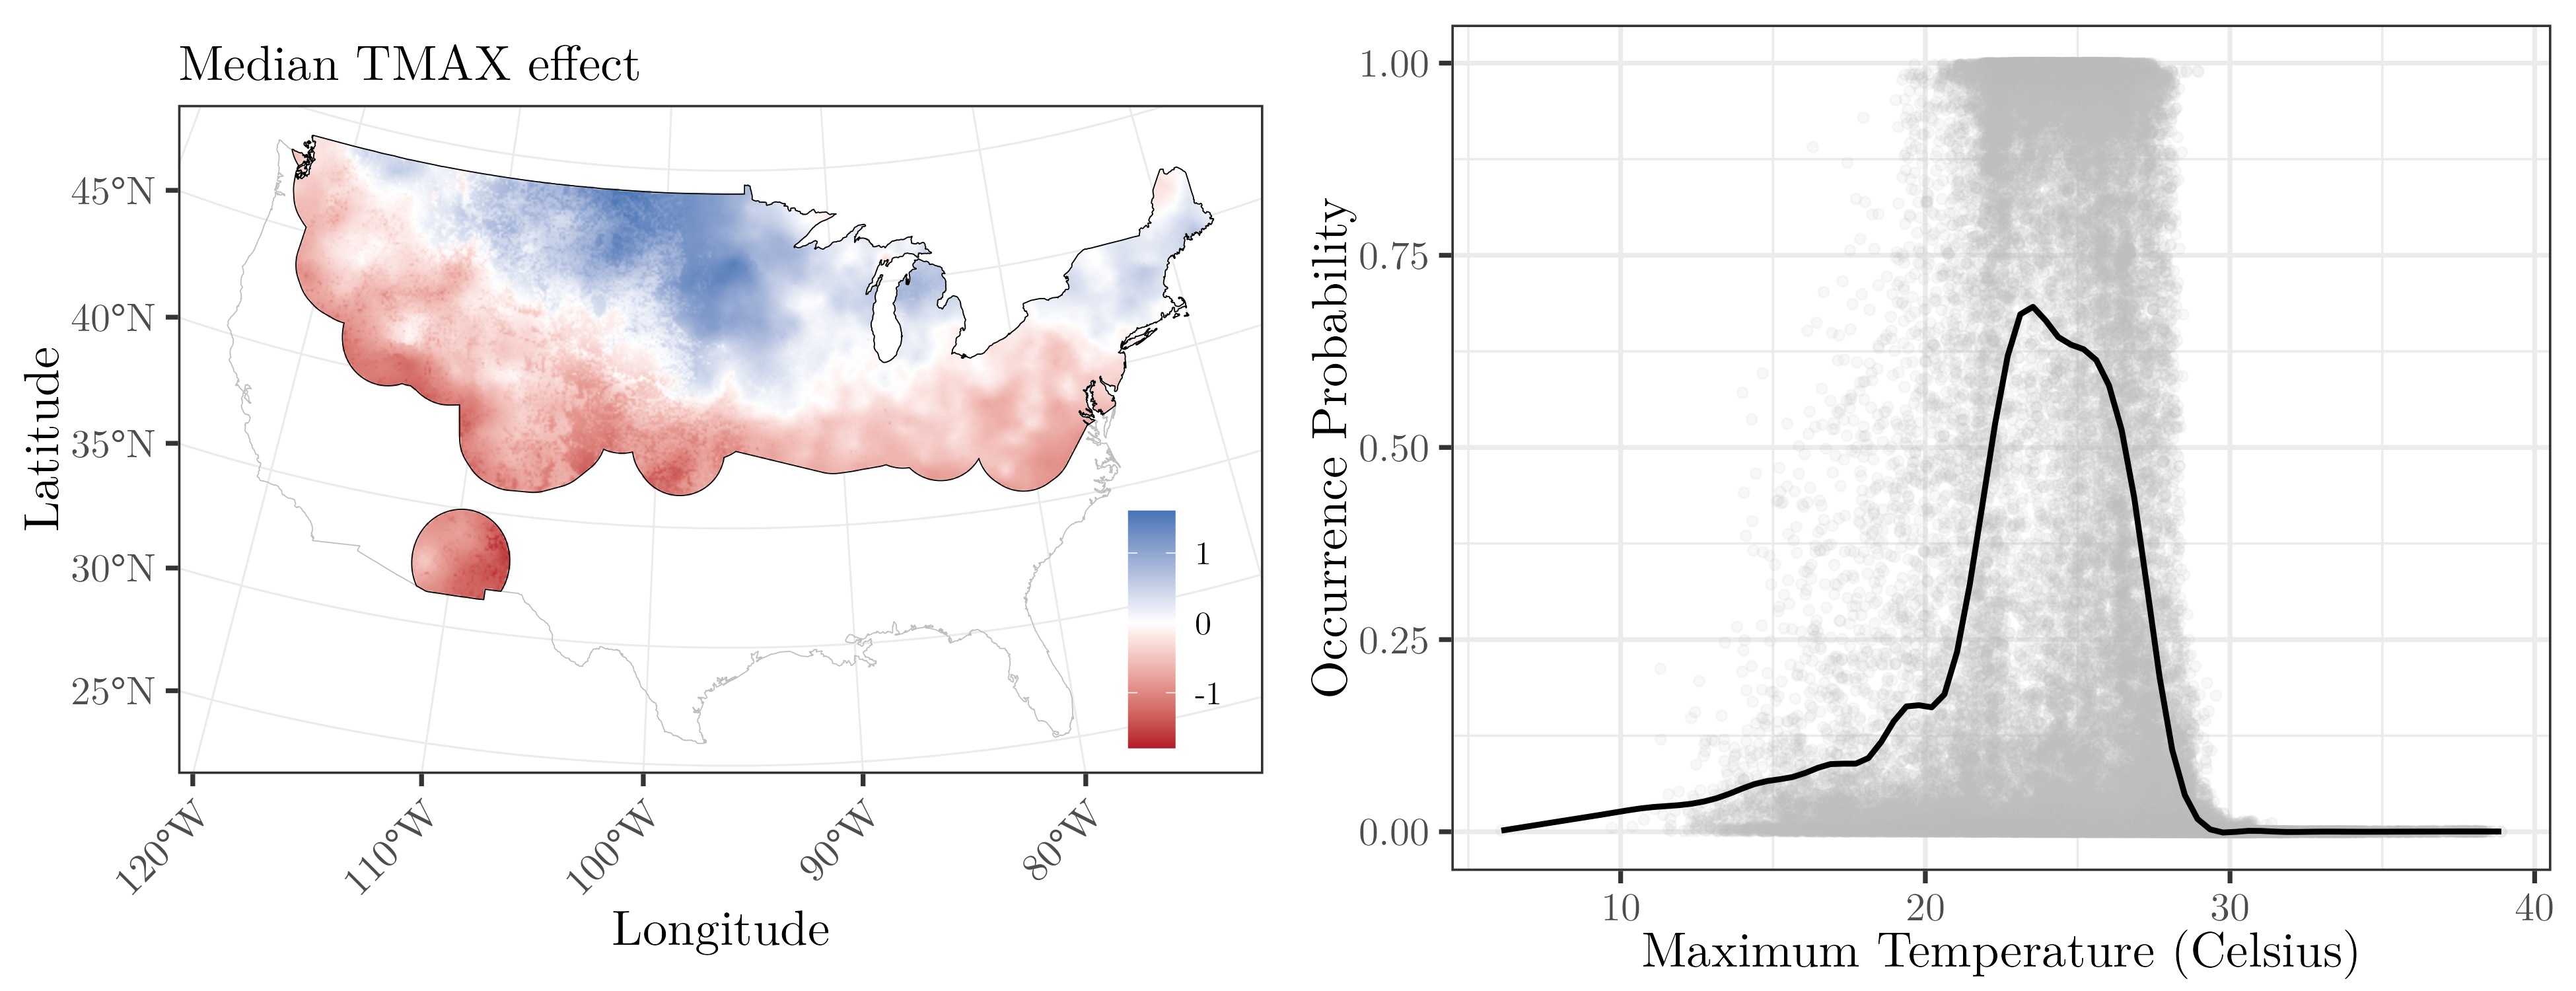
\includegraphics[width=11cm]{../figures/svc-bobolink.png}
\end{center}

\end{frame}

\begin{frame}{Software}

\begin{itemize}
    \item \texttt{spBayes}: univariate Gaussian SVC with full GPs
    \item \texttt{spOccupancy}: univariate Binomial SVC with NNGPs (multivariate on its way)
    \item \texttt{varycoef}: maximum likelihood Gaussian SVCs (Dambon et al. 2021 \textit{Spatial Stats.})
    \item \texttt{sdmTMB}: penalized likelihood and Bayesian SVC GLMMs (Anderson et al. 2022 \textit{bioRxiv})
\end{itemize}

\end{frame}

\begin{frame}{Exercise: 10-year occurrence trend of Wood Thrush}

\begin{itemize}
     \item Data come from USGS North American Breeding Bird Survey
     \item We desire to account for observational biases in detection of the birds (i.e., false negatives).
     \item Add on an additional observational layer to our hierarchical model
\end{itemize}

\begin{center}
   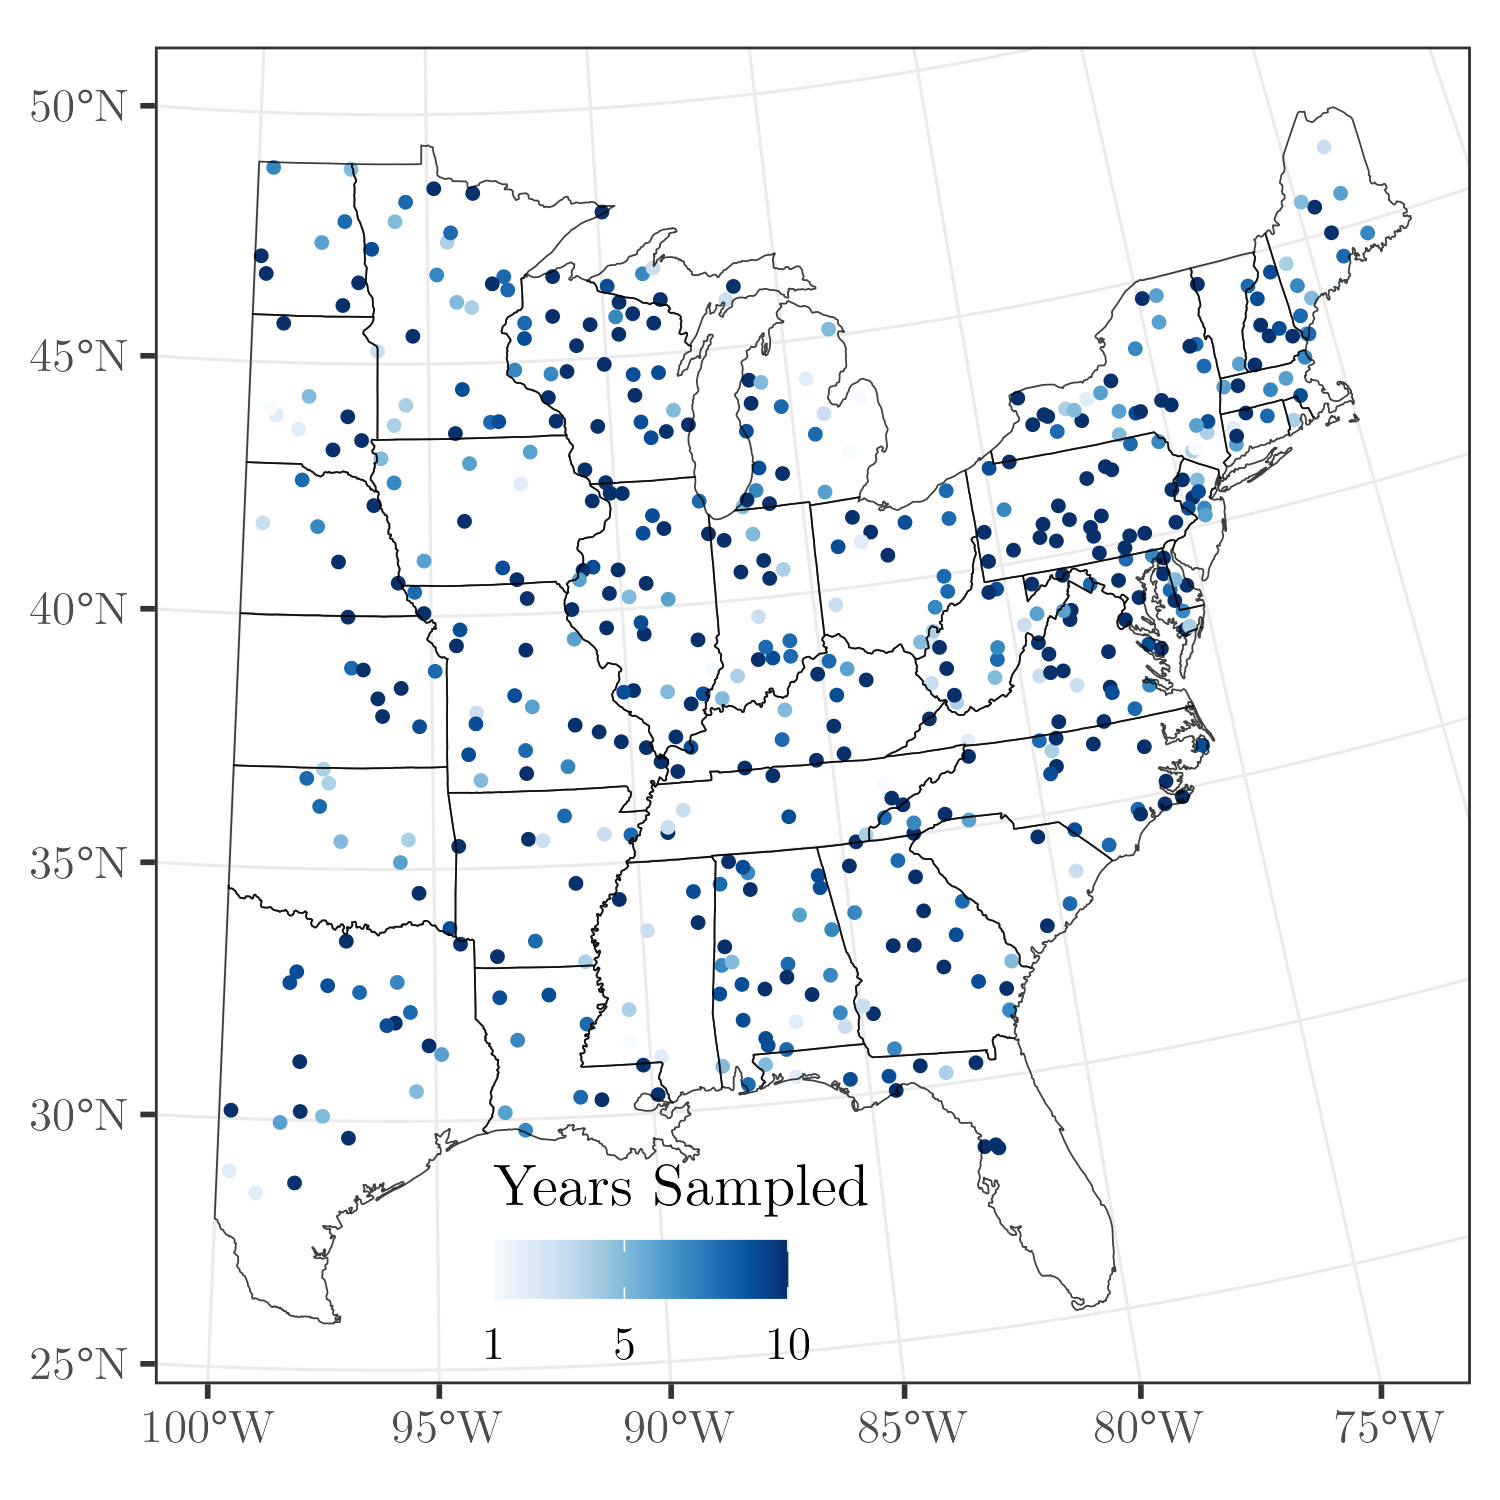
\includegraphics[width=5cm]{../figures/EAWP-data.png}
\end{center}

\end{frame}

\begin{frame}{Exercise: Process model}
  \begin{itemize}
          \item Let $z_t(\bs_i)$ denote the true presence (1) or absence (0) of the species at site $i = 1, \dots, 500$ during year $t = 1, \dots, 10$. \pause
	  \item If the bird was detected at a site and year, we know $z_t(\bs_i) = 1$. If not, it might be there and we just missed it during the surveys. \pause
	  \item We model $z_t(\bs_i)$ just as before with a Bernoulli GLM, with a SVC for trend
          \begin{align*}
		  z_t(\bs_i) &\sim \text{Bernoulli}(\psi_t(\bs_i)) \\
		  \text{logit}(\psi_t(\bs_i)) &= \tilde{\beta}_0(\bs_i) + \tilde{\beta}_1(\bs_i) \cdot \text{YEAR}_t
	  \end{align*}
          \item $\tilde{\beta}_0(\bm{s}_i)$ and $\tilde{\beta}_1(\bs_i)$ are modeled as independent SVCs with NNGPs
  \end{itemize}

\end{frame}
	 
\begin{frame}{Exercise: Observation model}
	\begin{itemize}
	  \item Let $y_{t, k}(\bs_i)$ denote the observed detection (1) or nondetection (0) of the bird at site $i$ during year $t$ and survey $k = 1, \dots, 5$. 
	  \item We model $y_{t, k}(\bs_i)$ conditional on the true presence/absence of the species $z_t(\bs_i)$
		  \begin{align*}
			  y_{t, k}(\bs_i) \mid z_t(\bs_i) &\sim \text{Bernoulli}(p_{i, t, k} \cdot z_t(\bs_i)) \\
			  \text{logit}(p_{i, t, k}) &= \alpha_{0, t} + \alpha_1 \cdot \text{DAY}_{i, t, k} + \alpha_2 \cdot \text{DAY}^2_{i, t, k}
		  \end{align*}
	  \item A key assumption for identifiability is that $z_t(\bs_i)$ does not change across the $5$ replicate surveys at site $i$ during year $t$.
	\end{itemize}
\end{frame}


\end{document}
